\begin{figure*}
  \begin{center}
    \begin{tabular}{c}
      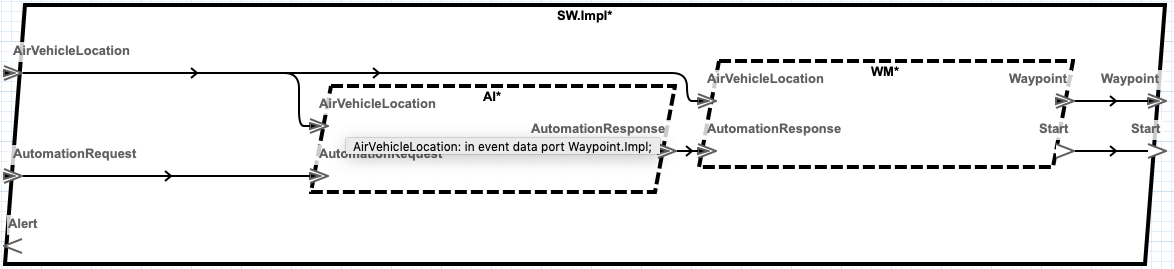
\includegraphics[scale=0.4]{example.png} \\
      (a) \\
      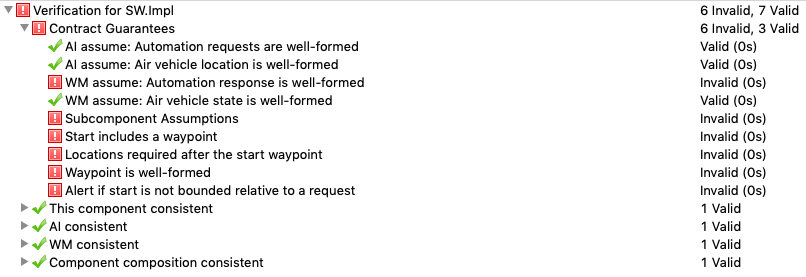
\includegraphics[scale=0.4]{example-certificate.png} \\
      (b)
    \end{tabular}
  \end{center}
\caption{Automated UAV route planning system. (a) Unhardened system. (b) Failure certificate.}
\label{fig:example}
\end{figure*}

\figref{fig:example} is an AADL model of an implementation of a software system (SW) for route planning and automated control for a UAV. It is loosely based on the system in the case study introduced later.  The source for the entire model is found at \cite{repo}. The system receives an automation request that is forwarded to an untrusted third-party route planner (AI) that decides the flight path of the UAV based on its current position and the requested task. The waypoint manager (WM) receives the mission command as a set of waypoints from the planner and starts the UAV flying the mission, issuing waypoints to the UAV flight controller as the UAV location changes. It is an \emph{as is} legacy component.

The expected behavior of the SW system, and the components in its implementation, are modeled with AGREE contracts. The contracts constrain input and state properties of output for component models. AGREE model checks this assume-guarantee system to hierarchically prove the composite system obeys all contract obligations under all possible finite input streams. 

The initial AGREE specification for the components and SW system make no assumptions about the integrity of the inputs and outputs. The cyber-vulnerability analysis identifies the potential of the untrusted AI route planner component to behave maliciously. As such, the AGREE specification for the AI route planner is updated to model this ability to behave maliciously as an untrusted component by removing any guarantees about its output; in other words, its output is unconstrained in the AGREE specification allowing it to take on any value and allowing it to send that value at any time.

The contracts for the other components are also updated with the threat analysis information. For example, the specification for the legacy waypoint manager adds assumptions about about its input being \emph{well-formed} since that is no longer known \emph{a priori} as AI route planner is now untrusted. 

Two requirements are added to the SW AGREE specification related to the cyber-vulnerability analysis: the first, \emph{Waypoint is well-formed} disallows malformed waypoints from being propagated downstream; and the second, \emph{Alert if start is not bounded relative to a request}, disallows a mission being started without a request or if the start is delayed more than one step after a request. Here the goal is to make clear that a delayed or unrequested automation response may prevent the UAV from flying its intended mission or to fly the wrong mission. 

AGREE examines the composition of the new specifications for the implementation in \figref{fig:example}(a) to determine whether it complies with the added cyber-resilience properties, by way of model checking. The results of the model checker are in \figref{fig:example}(b). The red exclamation points are properties that do not hold. Each comes with a counter-example. The results are not unexpected given the AI route planner's unconstrained behavior and the new assumptions about input to the legacy waypoint manager. The counter-example for \emph{Alert if start is not bounded relative to a request} shows a response in the first time step with no matching request. A clear malicious behavior from the untrusted component.

\begin{figure*}
  \begin{center}
    \begin{tabular}{c}
      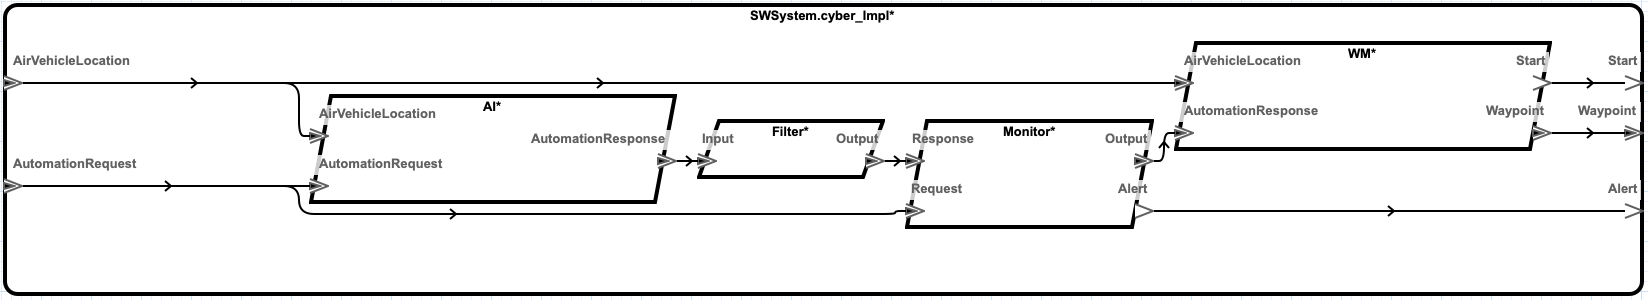
\includegraphics[scale=0.3]{hardened.png} \\
      (a) \\
      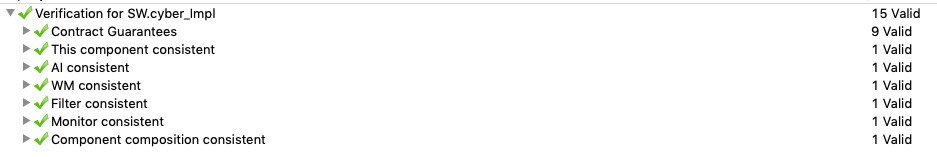
\includegraphics[scale=0.4]{hardened-certificate.png} \\
      (b)
    \end{tabular}
  \end{center}
  \caption{Hardened UAV system. (a) The implementation with high-assurance components. (b) Passing certificate.}
  \label{fig:hardened}
\end{figure*}

The system implementation is cyber-hardened by automatically transforming the model to insert high-assurance components in the form of a filter and a monitor as shown in \figref{fig:hardened}(a). A filter enforces an invariant over each datum in the data stream by not forwarding input to its output if that input is violating. The auto-generated AGREE specification states that only well-formed inputs are passed to the output. The user must provide this filtering policy, but it is usually based on the existing assumptions made by downstream components that consume the filter output. 

A monitor captures a relation over time on input data and is able to reason about temporal properties of that input. It raises an alert if ever the specified temporal properties are violated. The AGREE specification for the monitor states that an automation response can only be generated in conjunction with an automation request, and, also,  that response must come with the request or in the next step after the request. As with the filter, the user provides the policy, and that policy is based on the existing AGREE specification in the SW system.

The AGREE analysis of the cyber-hardened implementation with the auto-generated high-assurance components is shown in \figref{fig:hardened}(b). Here AGREE gives a proof certificate that the high-assurance components guarantee the correct behavior of the SW implementation in the presence of the considered cyber vulnerability from the untrusted AI route planner.

The high-assurance components are automatically synthesized from the AGREE specifications to equivalent models in the CakeML language. CakeML itself provides a complete verified compilation to binaries for several different platforms meaning that the resulting binaries exactly preserve the meaning of the original CakeML code \cite{cakeml}. 

A similar proof is given for the synthesis of the contract model for a high-assurance component to CakeML. A high-assurance component contract has a precise meaning in terms of data streams, and the synthesis exactly preserves that meaning in the generated code. In other words, for any set of input streams that meet the component's contract assumptions, the output streams produced from the synthesized CakeML exactly match the output streams from the high-assurance component's contract. 

Preserving the input/output relationship of streams between the two models lifts the contract verification results to the deployed system. If the contract model verifies, then the meaning of those results hold for the deployed system if the other components implement their contracts, an appropriate schedule exists that follows the dependent data-flow, and the communication fabric works as expected.